\scanpage{78}
\mspage{15}
6. Soit
\[
(44)\qquad P=(S,A,\unsure{\mathcal R|R}\subset S\times A)
\]
un polygône combinatoire fini d'ordre $n\geq3$,
\[
(45)\qquad D_P=D
\]
le groupe de ses automorphismes, $D_P^+=D^+$ le sous groupe d'indice $2$ des automorphismes conservant l'orientation, ou rotations,
\[
(46)\qquad 1\mathbin{-}D^+\mathbin{-}D\longrightarrow\{\pm1\}\longrightarrow1.
\]
On identifie l'ensemble $\underline\omega_P=\underline\omega$ des orientations de $P$ à l'ens. des deux générateurs privilégiés de $D^+$, \deleted{\unsure{considérés en tant qu'automorphismes}}
\[
(47)\qquad
\begin{array}{ccc}
\underline\omega&\subset&D^+\\
\Vert&&\\[-2pt]
\{\omega,\omega'\}&&
\end{array}
\]
de sorte que pour $\omega\in\underline\omega$, et pour $\forall\,s\in S,a\in A$, $\omega(s)$ est un sommet \uline{adjacent} à $s$, $\omega a$ une arête adjacente à $a$.

\uline{Il} existe un plongement, unique à \uline{isom.} unique, \deleted{$\unsure{\Sigma_P}$} de $S$ dans une sphère complexe, \inserted{$\Sigma=\Sigma_P$} \deleted{de} telle que les opérations de $D$ se prolongent en automorphismes complexes de $\Sigma_P$ :
\[
(48)\qquad S=S_P\hookrightarrow\Sigma=\Sigma_P:
\]
-- l'unicité est déjà garantie en exigeant le prolongement des opérations de $D^+$, qui implique celle des opérations de $D$ tout entier. Alors le polygône $P$ est réalisé canoniquement par des points de $\Sigma$ et des arcs de grand cercle de $\Sigma$, \deleted{\unsure{et}} tous \deleted{\unsure{derniers}} placés sur un même (grand) cercle,
\margin{\uline{NB} Cela marche sur $\forall$ corps alg. clos de car. première à $n$ -- plus gén. sur tout schéma de base sur lequel $\mu_n$ est un revêtement trivial... $\downarrow$}
\margin{La démonstration se fait en notant que \deleted{considérer}\inserted{\unsure{l'action de}} $D_P^+$ sur $\Sigma$ est \unsure{isom. à} l'action de $\mu_n\subset G_m$ sur $\Sigma_0=\mathbb P^1_{\mathbb C}$, \unsure{puis,} \uline{\unsure{Il}} \unsure{existe que} $\unsure{DPS}$ \unsure{que} \unsure{celle} \unsure{soit} $s_0\in S$, $\omega\in\underline\omega$, \unsure{d'où} $\unsure{\Phi}\longrightarrow\unsure{P_\omega}$, $\unsure{P_\omega}\longmapsto0$, $D_P\simeq D_n$. \unsure{aux} pôles $0,\infty$, \unsure{et isom.} $\unsure{R_0}$ \unsure{précisé} -- l'orbite de $D_P^+$ \unsure{fournit} \unsure{le point} $1$ \unsure{de} $\Sigma_P\simeq\mathbb P^1_{\mathbb C}$, \unsure{où} l'action \unsure{de} $\unsure{\gamma}$ \unsure{par multiplication} \unsure{par} $\unsure{\lambda}$, \unsure{et} \unsure{l'unique} \unsure{iso.} $\unsure{P_{\omega'}}\longmapsto\infty$, $\unsure{R_{s_0}}\longmapsto1$, \unsure{et} \unsure{pour} \unsure{cet isom.} l'action de $\unsure{\gamma}$ sur $\Sigma$ s'identifie à conjug. complexe...}
\figure{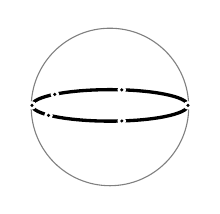
\begin{tikzpicture}[x=1cm,y=1cm]
\draw[gray,thin] (0,0) circle (1);
\draw[very thick] (0,0.02) ellipse (0.99 and 0.20);
\foreach \x/\y in {0.99/0.02,0.15/0.218,-0.7/0.16,-0.99/0.02,-0.78/-0.106,0.15/-0.178}
{\fill[white] (\x,\y) circle (0.055);\fill (\x,\y) circle (0.022);}
\end{tikzpicture}}
\margin{77}
